\documentclass[12pt]{article}
% Include packages
%%\usepackage[letterpaper]{geometry} 
\usepackage{amsmath,amssymb}
 \usepackage{graphicx}
 \usepackage{ifthen, comment}
% \usepackage{soul}
\usepackage{natbib} 
\usepackage{color}
\usepackage{fancyhdr}
\usepackage{hyperref}
%\hypersetup{pdftex, colorlinks=true, linkcolor=blue, citecolor=blue, filecolor=blue, urlcolor=blue, pdftitle=Stat216CoursePack, pdfauthor=Jim R-C, pdfsubject=, pdfkeywords=}

 \textwidth = 6.75 in
 \textheight = 9.75 in
 \oddsidemargin = 0.0 in
 \evensidemargin = 0.0 in
 \topmargin = -.4 in

\parskip = 0.2in
\parindent = 0.0in
\addtolength{\topmargin}{-.575in}
\addtolength{\oddsidemargin}{-.2in}
\addtolength{\evensidemargin}{-.275in}

\newcounter{alistctr}
\newenvironment{alist}{\begin{list}{\Alph{alistctr}.\ }
           {\usecounter{alistctr}}} {\end{list}}

\newsavebox{\fmbox}
\newenvironment{fmpage}[1]
{\begin{lrbox}{\fmbox}\begin{minipage}{#1}}
{\end{minipage}\end{lrbox}\fbox{\usebox{\fmbox}}}

%\input diagxy
%\xyoption{curve}
% Spacing and displaystyle
\newcommand{\ds}{\displaystyle}
\newcommand{\vs}[1]{\vspace{#1in}}
\newcommand{\hs}[1]{\hspace{#1in}}
\newcommand\textstyleInternetlink[1]{\textcolor{blue}{#1}}
\newcommand{\xb}{\overline{x}}
\newcommand{\phat}{\widehat{p}}

%\fancyhead[RE]{\textit{ \nouppercase{\leftmark}} }
%\fancyhead[LO]{\textit{ \nouppercase{\rightmark}} }

\fancypagestyle{plain}{ %
  \fancyhf{} % remove everything
  \renewcommand{\headrulewidth}{0pt} % remove lines as well
  \renewcommand{\footrulewidth}{0pt}
}
\includecomment{key}  
\includecomment{students} 
%% To make student version, uncomment this line:
\excludecomment{key}  
%% To run key, comment out this line instead:
%%\excludecomment{students} 

\begin{document}
 \begin{titlepage}
 \vspace*{1in}
 \begin{center}
 {\huge \sf   Stat 216 Course Pack Spring 2016}\\
\ \\
{ \LARGE \sf Activities and Notes }\\
  \ \\
  {\large\bf\  } \vspace{.2in}\\
  \ \\

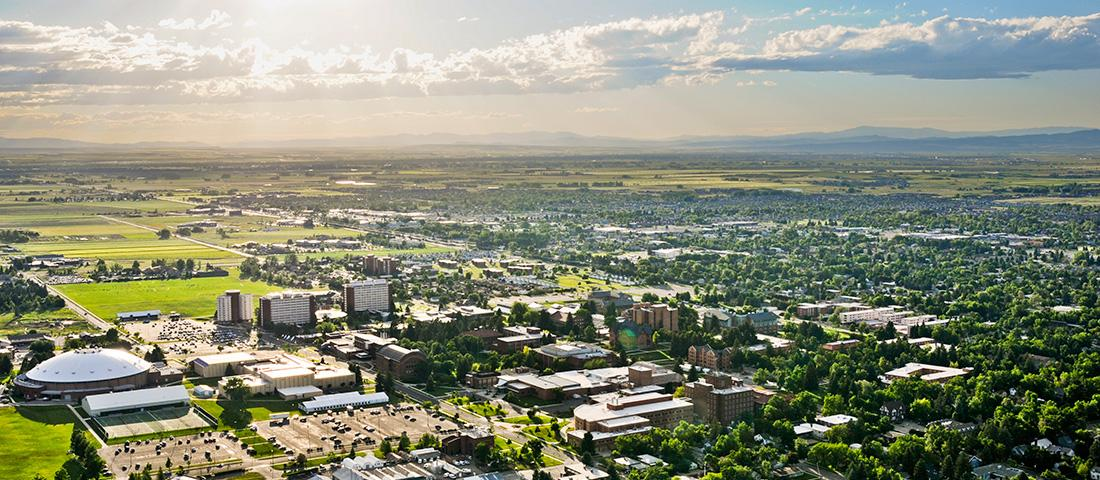
\includegraphics[width=.9\linewidth]{../MSU2NWpanorama.jpg}\\
\hspace*{\fill} {\tiny Photo by Kelly Gorham}\hspace*{.8cm}
\vspace{1in}

{\Large \sf
  Dr. Jim Robison-Cox\\
  Department of Mathematical Sciences\\
  Montana State University} \vfill 

{\small
 License: Creative Commons BY-SA 3.0
\url{https://creativecommons.org/licenses/by-sa/3.0/legalcode}  
}
\end{center}


 \end{titlepage}


%\newpage
\thispagestyle{empty}
%\thispagestyle{empty}

\begin{center}\tabcolsep=2pt
\vspace{-.5in}
{\LARGE \bf STAT 216 \hspace{.05in} Introduction to Statistics}
\\
{\Large \bf Spring 2016 Calendar of Topics}\\
for Sections  3, 6, 9, 11, 13, 15, 17, and 18  meeting Tuesdays and
Thursdays
\begin{tabular}{|c|c|} \hline
          &          \\
 \bf{TUESDAY} & \bf{THURSDAY} \\
\hspace{3.4in} & \hspace{2in}\\ \hline \hline
% Week 1
  & \bf{January}  \hfill\bf{14} \\
&Martian Alphabet \small{(1)}    \\
\multicolumn{2}{|c|}{\fbox{ \small\bf{Classes Begin January 13} }}  \\ \hline
% Week 2
  \hfill\bf{19} & \hfill\bf{21} \\
   Descriptive Stats \small{(2)} &
 \hfill      Sampling \small{(3)}\  \hfill \small{\sf B1} \\
\multicolumn{2}{|c|}{\fbox{  \small\bf{Jan 20: Last Day to Add
      On-Line} }}
 \\ \hline
% Week 3
  \hfill\bf{26} & \hfill\bf{28} \\
   Helper--Hinderer \small{(4)} &
 \hfill   Hyp Test 1 proportion(ESP) \small{(5)} \  \hfill  \small{\sf B2}  \\ 
\multicolumn{2}{|c|}{\fbox{  \small\bf{Jan 27: Last Day to Drop
      On-Line}}} \\ 
  \hline

% Week 4
   \bf{February}\hfill\bf{2} & \hfill\bf{4} \\
  Estimate 1 proportion \small{(6)}& 
 \hfill  What ``confidence'' means \small{(7)}\  \hfill \small{\sf B3} \\
\multicolumn{2}{|c|}{\fbox{  \small\bf{Feb 3: Last Day to Avoid a W} }}   \\
   \hline

% Week 5
  \hfill\bf{9} & \hfill\bf{11} \\
   MIT  \small{(8)} &  Unit  1 Review  \small{(9)}  \\ 
 \multicolumn{2}{|r|}{\fbox{\bf Feb 11: Common Hour Exam I 6:00 - 7:50
     pm  Rooms: TBA}}  \\
    \hline

% Week 6
  \hfill\bf{16}& \hfill\bf{18} \\
  Exp vs Obs study \small{(10)}& 
 \hfill  Textbook Cost -- CI for $\mu$  \small{(11)} \  \hfill  \small{\sf B4}\\ 
\hline 

% Week 7
  \hfill\bf{23} & \hfill\bf{25} \\
 Peanut Allergies \small{(12)} &  
 \hfill Weight Awareness $p_1 - p_2$ \small{(13)} \  \hfill \small{\sf B5}\\ 
 \hline

% Week 8
   \bf{March} \hfill\bf{1} & \hfill\bf{3} \\
 Energy Drinks $\mu_1 - \mu_2$ \small{(14)}&
 \hfill  Arsenic (Test $\mu_1$ )  \small{(15)}  \  \hfill  \small{\sf B6}\\
  &  (50 min class)\\
 \hline

%% Week 9
 \hfill\bf{8}  & \hfill\bf{10}  \\
  Types of Errors \small{(16)} & 
 \hfill  Correlation/slope \small{(17)}   \hfill  \small{\sf B7}\\
  (50 min class) & (50 min class)  
 \\ 
\hline

% Week 9
\multicolumn{2}{|c|}{\bf March 14-18 Spring Break}  %% 20
 \\ \hline

% Week 10
  \hfill\bf{22} & \hfill\bf{24} \\
    Regression test $\beta_1$ \small{(18)} & 
 \hfill    More regression   \small{(19)}    \hfill  \small{\sf B8}   
\\ \hline

% Week 11
  \hfill\bf{29} & \hfill\bf{31} \\
 Unit 2  Review   \small{(20)}&  
  No Class  %% Z and t intro
\\
 \multicolumn{2}{|l|}{\fbox{\bf March 29: Common Hour Exam II 6:00 -
     7:50 pm Rooms: TBA}} 
\\ \hline

% Week 12
{\bf April}    \hfill\bf{5} & \hfill\bf{7} \\
 Normal Distribution \small{(21)}  &
 \hfill  Z inference for p   \small{(22)}  \  \hfill \small{\sf B9}\\
 \hline

% Week 13
   \hfill\bf{12}  &  \hfill\bf{14}  \\
  Z inference for $p_1-p_2$  \small{(23)} &
 \hfill  t distributions - one mean  \small{(24)} \  \hfill  \small{\sf B10}
\\ & \hspace*{\fill}
  \fbox{ \small\bf{April 15: Last Day to Withdraw}} \\ \hline
 
% Week 14
 \hfill\bf{19} & \hfill\bf{21} \\
 t inference for $\mu_1- \mu_2$  \small{(25)} &
 \hfill Paired data \small{(26)}  \hfill  \small{\sf B11}
\\ \hline

% Week 15
 \hfill\bf{26} & \hfill\bf{28} \\
  Concussion Effects \small{(27)}
  & Review    \small{(28)}
\\
  &  \small\bf{ Last Day of Class}  \\ \hline

% Week 16
% Finals Week
  \multicolumn{2}{|c|}{\textbf{Final Exam Week: May 2 -- May 6 }} \\
  \multicolumn{2}{|c|}{\bf{ Common Hour Stat 216  Exam: 
      Wednesday, May 4, 10:00 -- 11:50 am Rooms: TBA}} \\
\hline

\end{tabular}
\vspace{.2in} \\
\end{center}




%\thispagestyle{empty}

\begin{center}\tabcolsep=2pt
\vspace{-.5in}
{\LARGE \bf STAT 216 \hspace{.05in} Introduction to Statistics}
\\
{\Large \bf Spring 2016 Calendar of Topics}\\
for Sections   1, 2, 4, 5, 7, 8, 10, 12, 14, and 16 meeting {\bf MWF}
\vspace{.1in}\\
\begin{tabular}{|c|c|c|} \hline
 && \\
  \bf{MONDAY} & \bf{WEDNESDAY} & \bf{FRIDAY}  \\
 \hline \hline
% Week 1
  & \bf{January}  \hfill\bf{13} &  \hfill\bf{15} \\
&Martian Alphabet \small{(1)}&   Descriptive Stats \small{(2)}   \\
& \small\bf{Classes Begin} &   \\ \hline
% Week 2
  \hfill\bf{18} & \hfill\bf{20} & \hfill\bf{22} \\
   MLK Jr day & 
     Sampling \small{(3)}&\\
\  \hfill \small{\sf Q1}  & \small\bf{ Last Day to Add On-Line} &  \\ \hline
% Week 3
  \hfill\bf{25} & \hfill\bf{27} & \hfill\bf{29} \\
 \hfill   Helper--Hinderer \small{(4)}   \hfill \small{\sf Q2}&
   Hyp Test 1 proportion(ESP) \small{(5)} &
   \\ 
 & \small\bf{Last Day to Drop On-Line} &  \\ 
  \hline
% Week 4
   \bf{February}\hfill\bf{1} & \hfill\bf{3} & \hfill\bf{5} \\
 \hfill  Estimate 1 proportion \small{(6)}\  \hfill \small{\sf Q3}& 
  What ``confidence'' means \small{(7)} & \\
  &\small\bf{ Last Day to Avoid a W} &   \\
   \hline
% Week 5
  \hfill\bf{8} & \hfill\bf{10} & \hfill\bf{12} \\
 \hfill   MIT  \small{(8)}\  \hfill \small{\sf Q4}&
   Unit  1 Review  \small{(9)} &
   Exp vs Obs Study\small{(10)} \\  
& \multicolumn{2}{|c|}{\fbox{\bf Feb 11: Common Hour Exam I 6:00 - 7:50 pm Rooms: TBA}}  \\
    \hline
% Week 6
  \hfill\bf{15}& \hfill\bf{17}& \hfill\bf{19} \\
  Presidents Day & 
  Textbook Cost -- CI for $\mu$  \small{(11)}
   &  \\ 
\hline 

% Week 7
  \hfill\bf{22} & \hfill\bf{24} & \hfill\bf{26} \\
 \hfill Peanut Allergies \small{(12)} \  \hfill \small{\sf Q5}&  
 Weight Awareness $p_1 - p_2$ \small{(13)}  &\\ 
 \hline

% Week 8
   \hfill\bf{29}& \bf{March} \hfill\bf{2} & \hfill\bf{4} \\
 \hfill  Energy Drinks $\mu_1 - \mu_2$ \small{(14)}\  \hfill \small{\sf Q6}
  & Arsenic (Test $\mu_1$ ) \small{(15)} 
  & \\
 \hline

%% Week 9
 \hfill\bf{7}  & \hfill\bf{9} & \hfill\bf{11}  \\   
 \hfill  Types of Errors \small{(16)} \  \hfill \small{\sf Q7}& 
  Correlation/slope \small{(17)} & 
 No Class
   \\ 
\hline

% Week 9
\multicolumn{3}{|c|}{\bf March 14-18 Spring Break}  %% 20
 \\ \hline
%% Energy Drinks, $\mu_1 - \mu_2$  \small{(13)}& 
% Week 10
  \hfill\bf{21} & \hfill\bf{23} & \hfill\bf{25} \\
 \hfill   Regression test $\beta_1$ \small{(18)}\  \hfill \small{\sf Q8}&
   More regression  \small{(19)} 
 & University Day
 \\ \hline
% Week 11
  \hfill\bf{28} & \hfill\bf{30}&{\bf April}  \hfill\bf{1} \\
 Unit 2  Review   \small{(20)}&  
  No Class &  Z and t intro  \small{(21)} 
\\
 \multicolumn{2}{|l|}{\fbox{\bf March 29: Common Hour Exam II 6:00 -
     7:50 pm Rooms: TBA}} & 
\\ \hline
% Week 12
   \hfill\bf{4} & \hfill\bf{6} & \hfill\bf{8} \\
 \hfill Normal Distribution \  \hfill \small{\sf Q9}&
  Z inference for p   \small{(22)} &
  \\
 \hline
% Week 13
   \hfill\bf{11}  &  \hfill\bf{13} &  \hfill\bf{15}  \\
 \hfill  Z inference for $p_1-p_2$  \small{(23)} \  \hfill \small{\sf Q10}&
  t distributions - one mean  \small{(24)} &
\\ & &
   \small\bf{Last Day to Withdraw} \\ \hline
 
% Week 14
 \hfill\bf{18} & \hfill\bf{20}  & \hfill\bf{22}\\
 \hfill t inference for $\mu_1- \mu_2$  \small{(25)}\  \hfill \small{\sf Q11} &
  Paired data \small{(26)}&
\\ \hline

% Week 15
 \hfill\bf{25} & \hfill\bf{27} & \hfill\bf{29} \\
 \hfill  Concussion Effects \small{(27)}\  \hfill \small{\sf Q12}
 &
 & Review    \small{(28)}
\\
  & & \small\bf{ Last Day of Class}  \\ \hline

% Week 16
% Finals Week
  \multicolumn{3}{|c|}{\textbf{Final Exam Week: May 2 -- May 6 }} \\
  \multicolumn{3}{|c|}{\bf{ Common Hour Stat 216  Exam: 
      Wednesday, May 4, 10:00 -- 11:50 am Rooms: TBA}} \\
\hline

\end{tabular}
\vspace{.2in} \\
\end{center}




 \textheight = 9.25 in

\def\theTopic{Syllabus }
\def\dayNum{1}
\def\unitNum{1}

\headheight = .75 in
\headsep = 0.2 in
\pagestyle{fancy}
\fancyhf{}
\fancyhead[LE,RO]{
   {\it \theTopic }\\
   {\it Unit \unitNum\  Activity \dayNum \ Page \thepage }
}
\setcounter{page}{1}
 \newpage
 
\def\theTopic{Intro \& Syllabus }
\def\dayNum{1}

\section{Stat 216 Intro and Syllabus Summer 2016}

\begin{center}
  {\bf People}
\end{center}
\begin{itemize}
\item Your Instructor: (Write contact info here) \vspace{5.5cm}
\item Student Success Coordinator:  Melinda Yager\\
     email: melinda.yager@montana.edu\hfill Office: Wilson 2-259 \hfill
     406-994-5344
%   \item Course Supervisor: Dr. Robison-Cox\\
%     email: jimrc@montana.edu \hfill  Office: Wilson 2-241 \hfill
%     406-994-5340
\end{itemize}


\begin{center}
  {\bf Course Materials}
\end{center}
  You need to buy the Stat 216  Course Pack from  the MSU
  Bookstore.  It will not work to use an old one from a friend.

  Other materials, such as readings and assignments 
  %D2Boxes (our word for  very important homeworks) 
  will be downloaded from D2L, so be
  sure you can log in to the MSU D2L (Brightspace) system:\\
   \url{https://ecat.montana.edu/}.  If you have problems, view the
   help on that page.

 There is a course web page
 \url{http://www.math.montana.edu/courses/s216/index.html} which contains
 \begin{itemize}
 \item this syllabus
 \item Web links \url{http://www.math.montana.edu/courses/s216/courseWebLinks.html}
 \item Data links \url{http://www.math.montana.edu/courses/s216/DataLinks.html}
 \end{itemize}

  {\bf Recommendation:}  In D2L you can click on your name, go to your
    account settings,  select  the ``Email'' tab, and set {\bf
      Forwarding Options} to send D2L mail to an account which you
    check more regularly.  We strongly recommend that you do this.  We
    might need to send out updates, and forwarding means you will not
    have to login in to D2L to get them.

  We will  use  online web applications,  so you need
  access to a computer.  You will work as a group of three and one of
  your group needs to bring a computer for each class meeting.\\
 
\newpage

 
{\bf Course Description }
 
Stat 216 is designed to engage you in statistics using a simulation
approach to inference based on web apps. Small group discussion
activities and daily assignments have been shown by the research to be
effective. Upon completion of this course, you should understand the
foundational concepts of data collection and of inference and you will
appreciate the fundamental role that statistics plays in all
disciplines.  In addition, statistical summaries and arguments are a
part of everyday life, and a basic understanding of statistical
thinking is critical to being an informed consumer of the numerical
information you will encounter on a daily basis.  You will be exposed
to numerous examples of real-world applications of statistics that are
designed to help you develop a conceptual understanding of statistics.
 
Note: this course will be a lot of work, and attendance every day is
{\bf really important} for your success. You will need to prepare for class
every day and to turn in assignments twice per week.

Please think seriously about this as you decide if this course is the
right fit for you.    

   \begin{center}
     {\bf Learning Outcomes for STAT 216 }
   \end{center}
   \begin{itemize}
   \item Understand how to describe the characteristics of a distribution.
   \item Understand how data can be collected, and how data collection
     dictates the choice of statistical method and appropriate
     statistical inference.
   \item Interpret and communicate  interval estimates and
     hypothesis tests in the context of a problem. We will cover tests
     and estimation in the contexts of: one proportion, one mean, two
     proportions, two means, and a regression slope.   
   \item Understand when we might make causal inference from a
     sample to a population.
   \item Understand how selection of a sample influences the
     group to which we might make inference.
   \end{itemize}
    
{\bf CORE 2.0}:  This course fulfills the Quantitative Reasoning (Q)
CORE 2.0 requirement because learning statistics allows us to
disentangle what's really happening in nature from ``noise'' inherent in
data collection. It allows us to evaluate claims from advertisements
and results of polls and builds critical thinking skills which form
the basis of statistical inference.   

{\bf Comments and concerns}: We are always looking for ways to improve
this class and we want students to be successful.  The first step is
to discuss your comments or concerns with your instructor.  If they
are not resolved, contact the Course Supervisor, Melinda Yager. 


\newpage
 
{\bf Prerequisites }
 
You should have completed  a 100-level math course (or equivalent) with
a grade of C- or better (Alternatives: a good score on Math portion
of SAT or ACT, or a 3.5 on the MPLEX exam).   
 You should have familiarity with computers and technology (e.g.,
Internet browsing, word processing, opening/saving files, converting
files to PDF format, sending and receiving e-mail, etc.). See the
Technology section of the syllabus for more details.  
 


{\bf Technology} \vspace{-.3in}
\begin{itemize}
\item {\bf Web Applets}  We will be utilizing web applets 
 at \webAppURLFrst\ or
 if those are unavailable use the site: \webAppURLScnd.\\
  These run in a web browser, but
  may have trouble with older versions of the Microsoft IE browser.
\item {\bf Technology Policy}:  This course utilizes technology
  extensively.  You will need at least one laptop within your group each
  day.
\item {\bf Appropriate Use}: We need to use web apps, but it is NOT OK
  to use other websites during class. {\bf You may not I-chat or text
    with friends or  use web sites other than those we direct you to
    during class.} Our class time is really limited. We need to use it
  for group work and for instructors to give intros, wrapups, and
  reviews.  Students who use technology inappropriately will lose
  attendance or RAT points for the day, and will have to  leave the
  room if they cannot stop such behavior.
\item {\bf Turn OFF your cell phone and put it away}.
\end{itemize}

{\bf Math Learning Center} in 1-112 Wilson Hall is a very important
resource providing  help on Stat 216 topics.
%spring:
 % It is open every day, into the evenings on MTWR, and closes early on
 % Friday.
% summer
 It is open from 9:00 am to 1:30 pm Monday through Thursday in summer. 


{\bf Assessment}\\
Your grade in this course will be based on the following: 
\begin{itemize}
\item  {\bf Assignments: 25\%} %{\bf D2Boxes: 15\%}  
  These assignments  will help you learn
  the course material and software through 
  reflection and practice and are essential preparation for the exam. 

  Format: Your instructors will tell you if you submit these as
  electronic files uploaded to a D2L Dropbox or as hard copies. If electronic,
  it needs to be in a format we can read.  Adobe pdf is our standard.
  Submissions we can't read will not count.

% \item {\bf D2Quizzes:  10\%} These are similar to the D2Box
%   assignments, but are graded automatically (mostly) on D2L.

\item {\bf Midterm Exam \  30\%}
  %Common Hour Exam I, February 11, 2016, 6:00 pm: \hfill 20\%}\\  
  Taken individually, not in groups. You may bring one handwritten
  page of notes.  

% \item {\bf Common Hour Exam II, March 29, 2016, 6:00 pm: \hfill    20\%}\\
%   Taken individually, not in groups. You may bring a one handwritten sheet
%   of notes. 

\item {\bf Final Exam %May  2016: \hfill 25\%}.\\
               \  35\%}.\\
  This exam will be cumulative in content. Again, you will be allowed
  to bring in one page of handwritten notes for the final exam.   
 
\item {\bf Attendance/Participation/Preparation:  10\%} . Class
  participation is an important part of learning, especially in
  courses like this one that involve group cooperation.    

  {\it Participation/Attendance}: Students can miss class/arrive
  late/leave early once (1 day) before they will be penalized for
  non-participation due to an absence.  For each day missed
  thereafter, the students’ overall grade will be reduced 1\% (up to
  5\%).   In addition to attending, it's critically important that
  each student participates in class. Lack of participation can result
  in the same penalty as absence.
 %%Summer only:

  Online students are expected to spend an equivalent amount of time
  in the course ``Chat Room''. 


  {\it Preparation}: The in-class activities and out-of-class assigned
  readings  and videos are the primary source of  information for this course.
  Take them seriously, work through them with care.
  As a way to provide further emphasis to the
  activities and readings, most classes will include a Readiness
  Assessment Test (RAT) with questions covering the previous class's
  activity and readings required for the class.   
\end{itemize}

{\it Late or Missed Work}:  If you cannot be in class, it is your 
responsibility to notify the instructor and your group members with as
much advance warning as possible. In general, make-up exams or late
homework assignments will not be allowed. Case-by-case exceptions may
be granted in only extreme cases at the discretion of the
instructor (daily work) or Student Success coordinator (exams). You
must provide documentation explaining your absence for 
the instructor to determine whether an exception should be granted. If
you fail to provide documentation as requested then you will not be
able to make-up missed work at all.   
 
  Letter grades will be assigned using a 10 point scale.
  As an approximation (which will be fine tuned at the end of the semester)
  94 - 100 = A,  90 to 93 = A-, 87 to 89 = B+, etc.
 
{\bf Planning Ahead:}  In our experience, it takes 6 to 9 hours per
week outside of class to achieve a good grade in Stat 216.  By ``good'' we
mean at least a C because a grade of C- or below does not
count toward fulfilling degree requirements.  Many of you set your
goals higher than just getting a C, and we fully support that.  You
need roughly nine hours per week to  review past activities, read
feedback on previous assignments, complete current assignments, and
prepare for the next day's class. 
\\ 
{\bf Summer} merits a special warning -- each week is like three weeks
of a spring or fall semester.  You really need to spend time with this
material -- at least 20 hours per week.  

The Math Sciences office cannot accept assignments and cannot provide
information about grades (you can check on D2L -- they can't).


\begin{center}
{\large\bf University Policies and Procedures }  
\end{center}

{\bf Behavioral Expectations }\\
Montana State University expects all students to conduct themselves as
honest, responsible and law-abiding members of the academic community
and to respect the rights of other students, members of the faculty
and staff and the public to use, enjoy and participate in the
University programs and facilities. For additional information
reference see MSU's Student Conduct Code at: 
\url{http://www2.montana.edu/policy/student_conduct/cg600.html} .
Behavioral expectations and student rights are further discussed at:
\url{http://www.montana.edu/wwwds/studentrights.html} . 
 

 {\bf Collaboration }\\
Discussing assignments with others (in your group for example) is a
good way to learn.  Giving others answers is not doing them a favor,
because then they aren't learning the material.  Copying from others
is cheating, and will not be tolerated.  
University policy states that, unless otherwise specified, students
may not collaborate on graded material. Any exceptions to this policy
will be stated explicitly for individual assignments. If you have any
questions about the limits of collaboration, you are expected to ask
for clarification. 


 {\bf Plagiarism  }\\
Paraphrasing or quoting anothers work without citing the source is a
form of academic misconduct. Even inadvertent or unintentional misuse
or appropriation of anothers work (such as relying heavily on source
material that is not expressly acknowledged) is considered
plagiarism. If you have any questions about using and citing sources,
you are expected to ask for clarification. 

 {\bf Academic Misconduct  }\\
Section 420 of the Student Conduct Code describes academic misconduct
as including but not limited to plagiarism, cheating, multiple
submissions, or facilitating others’ misconduct. Possible sanctions
for academic misconduct range from an oral reprimand to expulsion from
the university. 

Section 430 of the Student Code allows the instructor to impose the
following sanctions for academic misconduct: oral reprimand; written
reprimand; an assignment to repeat the work or an alternate
assignment; a lower or failing grade on the particular assignment or
test; or a lower grade or failing grade in the course.  

 {\bf Academic Expectations  }\\
Section 310.00 in the MSU Conduct Guidelines states that students
must:\vspace{-.15in}
\begin{list}{}{}
\item[A.] be prompt and regular in attending classes;
\item[B.] be well prepared for classes; 
\item[C.] submit required assignments in a timely manner;
\item[D.] take exams when scheduled;
\item[E.] act in a respectful manner toward other students and the
  instructor and in a way that does not detract from the learning
  experience; and 
\item[F.] make and keep appointments when necessary to meet with the
  instructor.  
In addition to the above items, students are expected to meet any
additional course and behavioral standards as defined by the
instructor. 
\end{list}

  {\bf Withdrawal Deadlines  }\\
% January 27, 2016 is the last day to withdraw without a ``W'' grade.
 University policy is explicit that the adviser and instructor must
 approve requests to withdraw from a course with a grade of ``W''. 
 Students who stop attending and stop doing the work are not
 automatically dropped.  Taking a ``W'' does not hurt your GPA but it
 is a sign that you are not making progress toward your degree, and
 could affect your financial aide or student loans. 

% \newpage

 {\bf Group Expectations }\\
 We have all been in groups which did not function well.  Hopefully,
 we've also all had good experiences with working in groups.  Our use
 of groups in this course is based on educational research which
 provides strong evidence that working in groups is effective and helps
 us learn.  By expressing your opinions and catching each others
 mistakes, you will learn to communicate statistical concepts.  These
 are partly ``common sense''
 ideas (for instance, gathering more data provides a better foundation
 for decision making),  but they are often  phrased in
 odd ways. We find it really helps to talk about them  with
 others. 

% Your instructors will assign groups and will lead you through an
% activity to get to know each other. We'd like your honest opinions
% about what you need from your group and what you fear about working
% with a group.


\newpage
 \def\theTopic{Martian Alphabet}


\subsection{  Martian Alphabet }


How well can humans distinguish one ``Martian'' letter from another?
In today's activity, we'll find out.
When shown the two Martian letters, kiki and bumba, write down whether
you think bumba is on the left or the right. \vspace{.5cm}


When your instructor  tells you which is correct, write down whether
you got it right or wrong. \vspace{.5cm}


\begin{enumerate}
\item  If humans really don't know Martian and are just guessing, what
  are the chances of getting it right? 
\begin{students}
  \vspace{1cm}
\end{students}    
\begin{key}
   {\it one-half.}
\end{key}
 
  \item We will assume that humans are just guessing. Discuss with
    your group: How can the three of you use  coins and the ``just
    guessing'' assumption to mimic  the number of people in a group
    of three who would get the right answer just by chance?
\begin{students}
  \vspace{1.5cm}
\end{students}    
\begin{key}
   {\it Each person flips a coin once (or 3 times) and we count the
     number of heads.}
\end{key}
 
\item  \label{flip3} We will now gather some data.  Each of you will
  flip a coin 3 times and record the number of Tails.  Sketch a plot
  of the numbers of Tails everyone got. The number of Tails will
  represent the number of right guesses of the Martian letters in
  three attempts.   
\begin{students}
  \vspace{3cm}
\end{students}    
\begin{key}
   {\it Probabilities for 0, 1, 2, 3 are 1/8, 3/8, 3/8, 1/8, so we
     hope to see that an outcome of 3 rights should happen about 1/8th
   of the time.}
\end{key}

\item Our class of thirty-some students might not give a clear picture
  of the distribution.  Your instructor will use a web app to get
  several 1000 trials.  Sketch the distribution here. 
\begin{students}
  \vspace{3cm}
\end{students}   

\item Now return to the `bumba' results and count the CORRECT bumba
  results in your group.  Is your group particularly good or bad at
  Martian? How do you tell?
\begin{students}
  \vspace{1cm}
\end{students}    
\begin{key}
   {\it good, we hope relative to the ``just guessing'' coin flips.}
\end{key}


  \item Let's collect more data, because just 3 people do not provide 
    much information.  We want to combine 3 or 4 groups (as instructed) to have
    9 or 12 of your responses. What will change from \# \ref{flip3} above? \\
    \begin{enumerate}
    \item Each flip a coin \underline{\hspace{.5in}} 
\begin{key}
   {\it \underline{9 or 12}}
\end{key}
        times to see
      what would happen under the ``just guessing'' scenario. 
    \item Change the spinner app to get the right  distribution.
\begin{students}
  \vspace{2cm}
\end{students}    
\begin{key}
   {\it Keep 2 outcomes: Success and Failure at 50/50 chance of each,
     but change [Last Spin] to 12. Run several 1000 trials. }
\end{key}
   

\item Sketch the distribution. Your instructor will pick 9 or 12 students
  to see how unusual their `bumba' answers are relative to the
  ``just guessing'' spinner results. Where does their number
  correct fall?
\begin{students}
  \vspace{3cm}
\end{students}    
\begin{key}
   {\it I got one 11 and no 12's out of 1000 spins. I expect students
     to get 11 or 12 correct.}
\end{key}
    \end{enumerate}


\item Finally, we'll use data from the whole class. 
    \begin{enumerate}
    \item How do we change the spinner app to get the correct
      distribution?  Sketch it here.
\begin{students}
  \vspace{4cm}
\end{students}    
\begin{key}
   {\it Keep 2 outcomes: Success and Failure at 50/50 chance of each,
     but change [Last Spin] to class size. Run several 1000 trials. }
\end{key}

\item  How unusual are the classes   answers relative to the ``just guessing'' spinner results?
\begin{students}
  \vspace{2cm}
\end{students}    
\begin{key}
   {\it Way out in the tail, I hope.}
\end{key}
\end{enumerate}
\item  Is it possible that we could see results this extreme just by
  chance?
\begin{students}
  \vspace{2cm}
\end{students}    
\begin{key}
   {\it Yes.}
\end{key}

\item Does this activity provide strong evidence that we were not just
  guessing at random?  If so, what do you think is going on here?
\begin{students}
  \vspace{2cm}
\end{students}    
\begin{key}
   {\it  Yes. View the TED talk to see why we can guess so well.}
\end{key}
  
\end{enumerate}


\begin{center}
  {\bf Take Home Messages}
\end{center}
  \begin{itemize}
  \item In this course we will learn how to evaluate a claim by
    comparing observed results (classes guesses) to a distribution.

  \item Blind guessing between two outcomes will be correct only
    about half the time. We can create data ( via computer simulation)
    to fit the assumption of blind guessing.

  \item Unusual results will make us doubt the assumptions used to
    create the distribution.  A large number correct is evidence that
    a person was not just blindly guessing.
  \end{itemize} \vspace{\fill}

{\bf Assignment}
\begin{itemize}
\item  Trade contact info with your group members.  Decide who will
  bring a computer to the next class.
\item   Purchase a copy of the course pack.
\item   Log in to this course on D2L. Set message forwarding to an
  account you read daily.
\item Watch videos assigned on D2L.
%\item View videos 1a through 1e posted on the Videos Link of D2L.
%\item Complete {\bf D2Quiz 1} on D2L by 11 pm Jan 18.  Note: you can
%  save a Quiz and work on it several times, but you may only submit it
%  once. %% Due Friday?
\item Read the Syllabus and ``Readings 1'' %on pages 1--5 and 9--12 
  for  the next class. You will be quizzed over them. 
\end{itemize}


Reference for ``Martian alphabet'' is a TED talk given by Vilayanur
Ramachandran in 2007. The synesthesia part begins at roughly 17:30 minutes.
\url{http://www.ted.com/talks/vilayanur_ramachandran_on_your_mind}  % Script: 3 pgs
 \newpage

\end{document}
